%!TeX root=../../tcc.tex

\chapter{Máximo Cinético}
Agora, considere o seguinte problema cinético. São dados $n$ pares
de valores em que cada par $(x_0, v)$ representa um valor que está
mudando linearmente com o tempo, assim como na lista cinética. Num
instante arbitrário $t \geq 0$, o valor correspondente ao par $(x_0,
v)$ é $x_0 + tv$. Desta vez, o objetivo é responder consultas mais
simples, do tipo: quem é o elemento com maior valor da coleção no
instante corrente.

Utilizando o mesmo exemplo da lista, se tivermos quatro elementos na
coleção, digamos $\left(6, -\dfrac{1}{2}\right)$, $(5, 0)$,
$\left(3, \dfrac{1}{4}\right)$ e $\left(0, \dfrac{4}{3}\right)$,
podemos representar essa coleção da seguinte maneira:

\begin{figure}
    \centering
        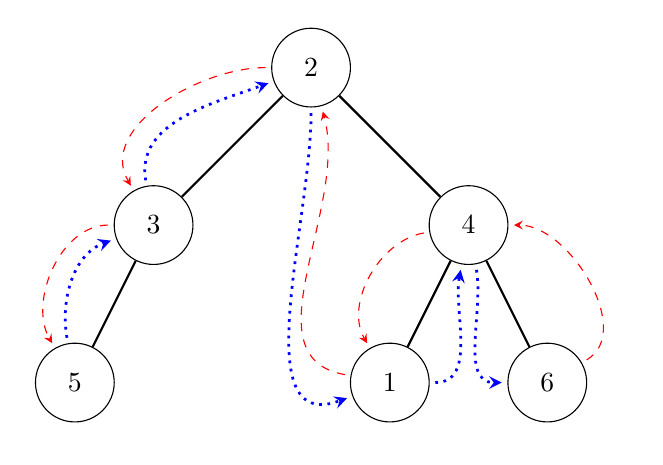
\begin{tikzpicture}[baseline=-2.25cm]
            \node[circle,draw,minimum size=1cm] (1) at (0,0)  {$2$};
            \node[circle,draw,minimum size=1cm] (2) at (-2,-2){$3$};
            \node[circle,draw,minimum size=1cm] (3) at (2,-2) {$4$};
            \node[circle,draw,minimum size=1cm] (4) at (-3,-4){$5$};
            \node[circle,draw,minimum size=1cm] (5) at (1,-4) {$1$};
            \node[circle,draw,minimum size=1cm] (6) at (3,-4) {$6$};
            % \node[label={7},circle,draw,minimum size=1cm] (7) at (3,-4) {$8$};
            % \node[label={8},circle,draw,minimum size=1cm] (8) at (-4,-6) {$4$};
            % \node[label={9},circle,draw,minimum size=1cm] (9) at (-2,-6) {$1$};
            \tikzstyle{filho}=[thick]
            \tikzstyle{pred}=[->, shorten >= 2pt, shorten <= 2pt,
                    dashed, >=stealth, red]
            \tikzstyle{sucessor}=[->, shorten >= 2pt, shorten <= 2pt,
                    dotted, >=stealth, blue, line width=0.35mm]
            % \tikzstyle{p4}=[->, shorten >= 2pt, shorten <= 2pt, dotted, >=stealth]
            \draw[filho] (1) -- (2);
            \draw[filho] (1) -- (3);
            \draw[filho] (2) -- (4);
            \draw[filho] (3) -- (5);
            \draw[filho] (3) -- (6);
            \draw[pred] (6) edge[out=30,in=0] (3);
            \draw[sucessor] (3) edge[out=280,in=180] (6);
            \draw[pred] (3) edge[out=190,in=120] (5);
            \draw[sucessor] (5) edge[out=0,in=260] (3);
            \draw[pred] (5) edge[out=170,in=285] (1);
            \draw[sucessor] (1) edge[out=270,in=200] (5);
            \draw[pred] (1) edge[out=180,in=120] (2);
            \draw[sucessor] (2) edge[out=100,in=200] (1);
            \draw[pred] (2) edge[out=180,in=120] (4);
            \draw[sucessor] (4) edge[out=100,in=200] (2);
        \end{tikzpicture}
        \qquad
        \qquad
        \qquad
        \begin{tabular}{|c|c|}
            \hline
            $i$ & $x_0$ \\
            \hline
            $1$ & $6$ \\

            $2$ & $3$ \\

            $3$ & $2$ \\

            $4$ & $7$ \\

            $5$ & $-2$ \\

            $6$ & $14$ \\
            \hline
        \end{tabular}
        \caption[Exemplo de estrutura da ABB]{Exemplo de árvore em
            que a ordem dos elementos, do menor para o maior no
            instante $\now = 0$, é $5 - 3 - 2 - 1 - 4 - 6$. Os
            apontadores para o elemento anterior são representados
            pelas setas vermelhas tracejadas e os apontadores para o
            elemento posterior são representados pelas setas azuis
            pontilhadas.}\label{fig:abb:exemplo}
\end{figure}

Agora, além das operações \textsc{advance}$(t)$ e
\textsc{change}$(j, v)$, queremos dar suporte à nova operação:
\begin{itemize}
    \item \textsc{query\_max}$()$ $\rightarrow$ devolve o elemento
    cujo valor é o maior no instante atual.
\end{itemize}
%!TeX root=./maximo.tex

\section{Heap Cinético}
\label{heap:secao}
Um bom jeito de resolver o problema do máximo cinético é
manter uma fila de prioridades com os elementos da coleção.
Dessa maneira, o elemento que se encontra na raiz da fila
será o que possui o maior valor da coleção.
Para implementar a heap utilizaremos um vetor.

Inicialmente o vetor começa com os índices dos elementos
e construímos um heap de acordo com o valor de cada elemento
no instante $t = 0$, ou seja, com o valor $x_0$ de cada elemento.

Uma vez de posse do heap montado, construímos um certificado
para cada par $($filho, pai$)$ no heap. O $i$-ésimo certificado,
que se refere ao par das posições $i$ e $\floor{\dfrac{i}{2}}$,
consiste no instante de tempo em que o $i$-ésimo elemento
passará a ter um valor maior que o valor do
$\floor{\frac{i}{2}}$-ésimo elemento do vetor,
se esse instante for maior que o instante atual.
Do contrário, o certificado consiste em $+\infty$. % Esse valor do certificado é o seu \underline{prazo de validade}.

% Esses prazos de validade são os \underline{eventos} que causarão modificações no vetor que mantém os elementos ordenados pelo seu valor e consequentemente em alguns certificados.

Esses $n - 1$ certificados são colocados em uma fila de
prioridade $Q$, com o prazo de validade como chave. Estamos
interessados nos certificados com menor prazo de validade.

Para descrever a implementação das três operações, precisamos
estabelecer o nome das novas variáveis usadas. São elas:
\begin{enumerate}
    % \item $n$: o número de elementos dados;
    % \item $x_0$ e \textit{speed}: vetores com o valor e a velocidade inicial de cada um dos $n$ elementos;
    % \item \now: instante atual;
    \item \textit{heap}: vetor com os índices dos $n$ elementos
    formando um heap de acordo com o seu valor no instante
    \textit{now};
    \item \textit{cert}: vetor com os certificados, onde
    \textit{cert}$[i]$ guarda o certificado entre $i$ e
    $\floor{\dfrac{i}{2}}$, para $1 < i \leq n$.
    % \item \textit{Q}: fila de prioridade para os certificados.
\end{enumerate}

A interface da fila de prioridade que utilizaremos não se altera.

% Para implementar a operação updatePQ$(Q, i, t)$ em tempo logarítmico no número de elementos na fila de prioridade, é necessário utilizar um vetor adicional \textit{indQ} que guarda em \textit{indQ}$[i]$ a posição do $i$-ésimo certificado em $Q$.

Um evento está associado a um certificado $(i, t)$ que expira
no instante $t$. O tratamento do evento correspondente ao
certificado $(i, t)$ consiste em trocar de lugar os índices
armazenados nas posições $i$ e $\floor{\dfrac{i}{2}}$ do vetor
\heap, e recalcular o prazo de validade de até cinco certificados:
\begin{itemize}
    \item do $\floor{\frac{i}{2}}$-ésimo certificado, se $i > 1$;
    \item do $j$-ésimo certificado, se $i > 1$ e $j \leq n$,
    onde $j = 2\cdot \floor{\dfrac{i}{2}} + ((i + 1)\mod2)$
    é o irmão de $i$;
    \item do $(2i)$-ésimo certificado, se $2i \leq n$;
    \item do $(2i + 1)$-ésimo certificado, se $2i + 1 \leq n$.
\end{itemize}

O $i$-ésimo certificado também deve ser ajustado para $+\infty$.
Finalmente, é necessário fazer ajustes em $Q$, alterando a
chave dos certificados que sofreram alteração.

Novamente, na implementação da operação \textsc{event},
utilizaremos a rotina \textsc{update}$(i)$ que calcula a
nova validade $t$ do $i$-ésimo certificado, se $1 < i \leq n$,
e chama a rotina \textsc{updatePQ}$(Q, i, t)$.

\begin{algorithm}[H]
    \caption{Função \textsc{update}.} \label{max:update}
\begin{algorithmic}[1]
    \Function{update}{$i$}
        \If{$1 < i \leq n$}
            \State $t \leftarrow $
            \Call{expire}{$i,\floor{\frac{i}{2}}$}
            \State \Call{updatePQ}{$Q,i,t$}
        \EndIf
    \EndFunction
    % \LineComment{\Call{expire}{$i,j$} calcula a validade do certificado entre os elementos $i$ e $j$}
\end{algorithmic}
\end{algorithm}

\begin{algorithm}[H]
    \caption{Função \textsc{event}.} \label{max:evento}
\begin{algorithmic}[1]
    \Function{event}{}
        \State $i \leftarrow  $ \Call{minPQ}{$Q$}
        \While{\cert[$i$] = \now}
            \State \heap[$i$] $\leftrightarrow$
            \heap$[\floor{\frac{i}{2}}]$
            \State \Call{update}{$i$}
            \State \Call{update}{$\floor{\frac{i}{2}}$}
            \State \Call{update}{$2\cdot
            \floor{\frac{i}{2}} + ((i + 1)~mod~2)$}
            \State \Call{update}{$2i$}
            \State \Call{update}{$2i + 1$}
            \State $i \leftarrow  $ \Call{minPQ}{$Q$}
        \EndWhile
    \EndFunction
\end{algorithmic}
\end{algorithm}

\begin{figure}[H]
    \centering
    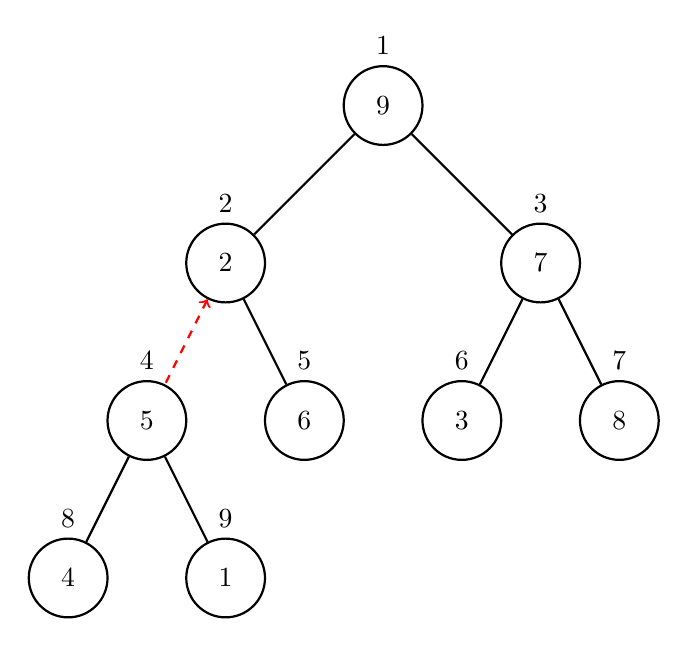
\begin{tikzpicture}[thick]
    \node[label={1},circle,draw,minimum size=1cm] (1) at (0,0) {$9$};
    \node[label={2},circle,draw,minimum size=1cm] (2) at (-2,-2) {$2$};
    \node[label={3},circle,draw,minimum size=1cm] (3) at (2,-2) {$7$};
    \node[label={4},circle,draw,minimum size=1cm] (4) at (-3,-4) {$5$};
    \node[label={5},circle,draw,minimum size=1cm] (5) at (-1,-4) {$6$};
    \node[label={6},circle,draw,minimum size=1cm] (6) at (1,-4) {$3$};
    \node[label={7},circle,draw,minimum size=1cm] (7) at (3,-4) {$8$};
    \node[label={8},circle,draw,minimum size=1cm] (8) at (-4,-6) {$4$};
    \node[label={9},circle,draw,minimum size=1cm] (9) at (-2,-6) {$1$};
        \tikzstyle{cert}=[<-, dashed, red]
        \draw[thick] (1) -- (2);
        \draw[thick] (1) -- (3);
        \draw[cert] (2) -- (4);
        \draw[thick] (2) -- (5);
        \draw[thick] (3) -- (6);
        \draw[thick] (3) -- (7);
        \draw[thick] (4) -- (8);
        \draw[thick] (4) -- (9);
        % \draw[->, color=red] (2) -- (3);
        % \draw[->] (3) -- (4);
        % \draw[->] (4) -- (5);
        % \draw[->] (1) edge (2) (2) edge (3) (3) edge (4) (4) edge (5)
    \end{tikzpicture}
    \caption{\cert[$4$] expirou.}
    \label{fig:maxdevent}
\end{figure}
\begin{figure}[H]
    \centering
    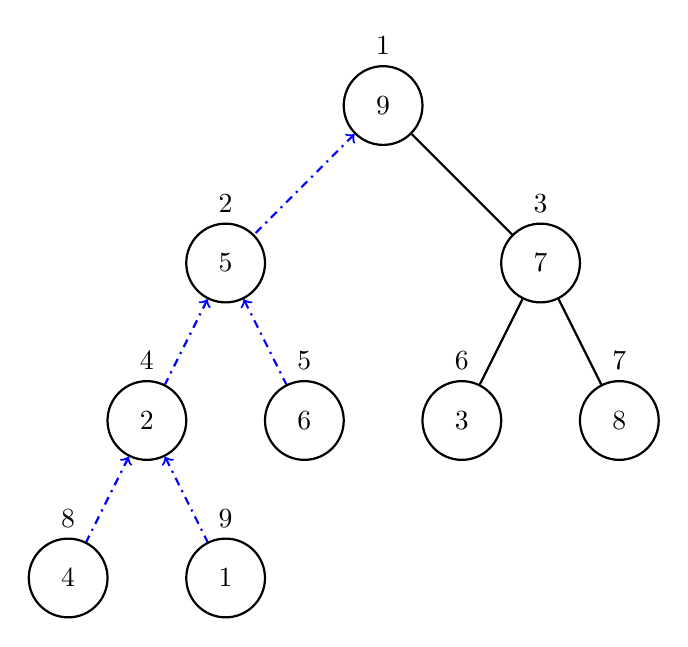
\begin{tikzpicture}[thick]
    \node[label={1},circle,draw,minimum size=1cm] (1) at (0,0) {$9$};
    \node[label={2},circle,draw,minimum size=1cm] (2) at (-2,-2) {$5$};
    \node[label={3},circle,draw,minimum size=1cm] (3) at (2,-2) {$7$};
    \node[label={4},circle,draw,minimum size=1cm] (4) at (-3,-4) {$2$};
    \node[label={5},circle,draw,minimum size=1cm] (5) at (-1,-4) {$6$};
    \node[label={6},circle,draw,minimum size=1cm] (6) at (1,-4) {$3$};
    \node[label={7},circle,draw,minimum size=1cm] (7) at (3,-4) {$8$};
    \node[label={8},circle,draw,minimum size=1cm] (8) at (-4,-6) {$4$};
    \node[label={9},circle,draw,minimum size=1cm] (9) at (-2,-6) {$1$};
        % \edef\pos{0}
        % \foreach \x in {1, 2,..., 5}{
        %     \pgfmathparse{\pos+2}
        %     \xdef\pos{\pgfmathresult}
        %     \node[circle,draw, minimum size=1cm] (\x) at  (\pos, 0) {$\x$};
        %     \node  at (\pos, -1) {$\x$};
        % }
        % \foreach \x [evaluate=\x as \y using int(\x + 1)] in {1, 2,..., 4}{
        %     \ifthenelse{\x==2}{\draw[->, draw=red] (\x) -- (\y);}{\draw[->, draw=black] (\x) -- (\y);}
        % }
        \tikzstyle{cert}=[<-, dashdotted, blue, thick]
        \draw[cert] (1) -- (2);
        \draw[thick] (1) -- (3);
        \draw[cert] (2) -- (4);
        \draw[cert] (2) -- (5);
        \draw[thick] (3) -- (6);
        \draw[thick] (3) -- (7);
        \draw[cert] (4) -- (8);
        \draw[cert] (4) -- (9);
        % \draw[->, color=red] (2) -- (3);
        % \draw[->] (3) -- (4);
        % \draw[->] (4) -- (5);
        % \draw[->] (1) edge (2) (2) edge (3) (3) edge (4) (4) edge (5)
    \end{tikzpicture}
    \caption{\heap[$4$] e \heap[$2$] foram trocados e \cert[$2$], \cert[$4$], \cert[$5$], \cert[$8$] e \cert[$9$] foram atualizados.}
    \label{fig:max:update}
\end{figure}

A operação \textsc{query\_max}$()$ consiste em devolver
\textit{heap}$[1]$, enquanto que a operação \textsc{change}$(j, v)$
consiste em alterar a posição $x_0[j]$ para
$x_0[j] + (\mathit{speed}[j] - v)\cdot now$,
a posição \textit{speed}[j] para \textit{v}
e recalcular os eventuais certificados de
que $j$ participa. Para tanto, a partir da
posição $i$ em que $j$ se encontra no vetor
\textit{heap}, podemos recalcular
\textit{cert}$[i]$ se $i > 1$, \textit{cert}$[2i]$ se
$2i \leq n$ e \textit{cert}$[2i + 1]$ se $2i + 1 \leq n$,
acionando a rotina \textsc{updatePQ} para fazer os devidos
acertos em $Q$ correspondentes a estas modificações.

\begin{algorithm}[H]
    \caption{Função \textsc{query\_max}.}
    \label{max:heap:query\_max}
\begin{algorithmic}[1]
    \Function{query\_max}{}
        \State \Return \heap$[1]$
    \EndFunction
\end{algorithmic}
\end{algorithm}

\begin{algorithm}[H]
    \caption{Função \textsc{change}.} \label{max:advance}
\begin{algorithmic}[1]
    \Function{change}{$j, v$}
        \State $x_0$[$j$] $\leftarrow x_0$[$j$]
        $+~($\speed[$j$] - $v)~\cdot~$\now;
        \State \speed[$j$] $\leftarrow v$
        \State \Call{update}{$i$}
        \State \Call{update}{$2i$}
        \State \Call{update}{$2i + 1$}
    \EndFunction
\end{algorithmic}
\end{algorithm}
\begin{figure}[H]
    \centering
    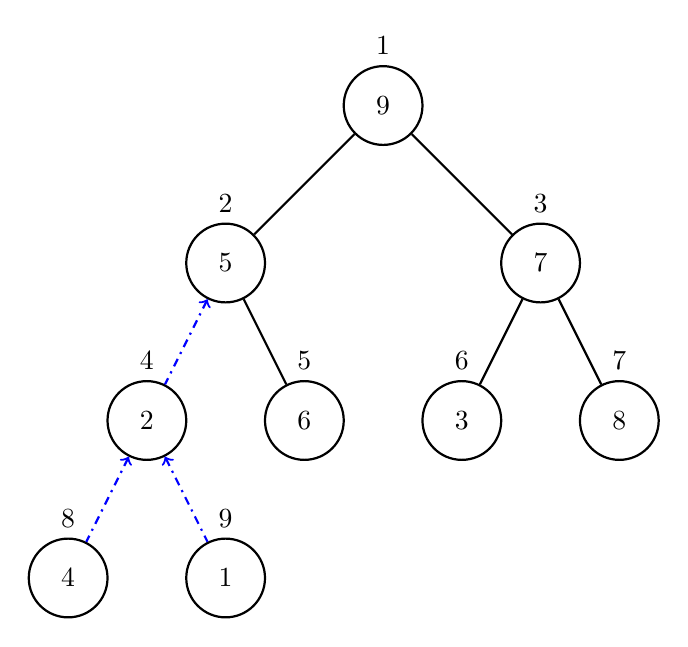
\begin{tikzpicture}[thick]
        \node[label={1},circle,draw,minimum size=1cm]
            (1) at (0,0) {$9$};
        \node[label={2},circle,draw,minimum size=1cm]
            (2) at (-2,-2) {$5$};
        \node[label={3},circle,draw,minimum size=1cm]
            (3) at (2,-2) {$7$};
        \node[label={4},circle,draw,minimum size=1cm]
            (4) at (-3,-4) {$2$};
        \node[label={5},circle,draw,minimum size=1cm]
            (5) at (-1,-4) {$6$};
        \node[label={6},circle,draw,minimum size=1cm]
            (6) at (1,-4) {$3$};
        \node[label={7},circle,draw,minimum size=1cm]
            (7) at (3,-4) {$8$};
        \node[label={8},circle,draw,minimum size=1cm]
            (8) at (-4,-6) {$4$};
        \node[label={9},circle,draw,minimum size=1cm]
            (9) at (-2,-6) {$1$};

        \tikzstyle{cert}=[<-, dashdotted, blue, thick]
        \draw[thick] (1) -- (2);
        \draw[thick] (1) -- (3);
        \draw[cert] (2) -- (4);
        \draw[thick] (2) -- (5);
        \draw[thick] (3) -- (6);
        \draw[thick] (3) -- (7);
        \draw[cert] (4) -- (8);
        \draw[cert] (4) -- (9);
    \end{tikzpicture}
    \caption{Após a mudança de velocidade do elemento 2,
    que se encontra em \heap[$4$], \cert[$4$], \cert[$8$] e
    \cert[$9$] foram atualizados.}
    \label{fig:predeventheap}
\end{figure}

%!TeX root=./maximo.tex

\newcommand{\thickness}{0.75mm}
\FloatBarrier
\section{Torneio cinético} \label{torneio:secao}

Considere o seguinte algoritmo para achar o valor máximo em um
conjunto de $n$ elementos: aloque um vetor \torneio~com $2n - 1$
posições. Inicializamos as últimas $n$ posições com os valores dos
$n$ elementos e uma variável $i$ com o valor da última posição, $i =
2n - 1$. Repita o seguinte processo até que $i$ seja igual a $1$: se
\torneio$[i] > $~\torneio$[i - 1]$, então
\torneio$\left[\floor{\frac{i}{2}}\right] =$~\torneio$[i]$, caso
contrário \torneio$\left[\floor{\frac{i}{2}}\right] =$~ \torneio$[i
- 1]$, e, por fim, subtraia~$2$ de $i$. Dessa maneira, ao fim da
execução do algoritmo, em \torneio$[1]$ estará o maior valor da
coleção. Na verdade, podemos fazer a comparação de maneira indireta,
e guardar os índices dos elementos no vetor \torneio~e não seus
valores. Veja a Figura \ref{fig:torneio:exemplo}.

Podemos pensar nessas comparações entre \torneio$[i]$ e
\torneio$[i-1]$ como sendo partidas de um torneio classificatório,
por isso o nome torneio. Chamaremos de ``partida'' as comparações
entre \torneio$[i]$ e \torneio$[i-1]$ e diremos que o elemento~$j$
``vence'' o elemento $k$ quando os elementos $j$ e $k$ disputaram
uma partida entre si e o elemento $j$ possuía maior valor nesse
instante. Utilizaremos esse ``torneio'' para resolver o problema do
máximo cinético e, para implementá-lo, será utilizado um vetor como
o citado no algoritmo acima.

\begin{figure}
    \centering
        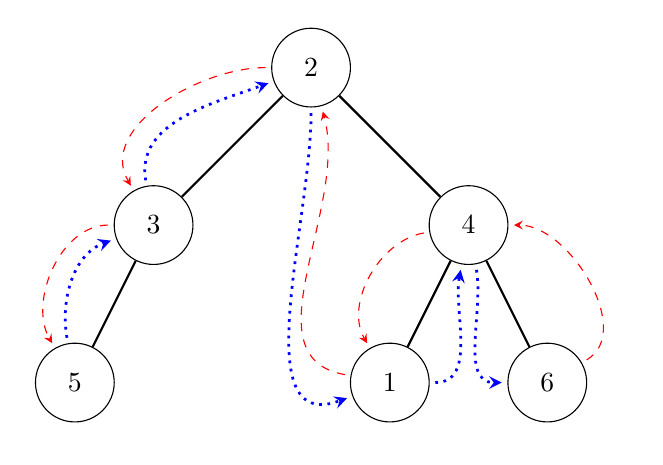
\begin{tikzpicture}[baseline=-2.25cm]
            \node[circle,draw,minimum size=1cm] (1) at (0,0)  {$2$};
            \node[circle,draw,minimum size=1cm] (2) at (-2,-2){$3$};
            \node[circle,draw,minimum size=1cm] (3) at (2,-2) {$4$};
            \node[circle,draw,minimum size=1cm] (4) at (-3,-4){$5$};
            \node[circle,draw,minimum size=1cm] (5) at (1,-4) {$1$};
            \node[circle,draw,minimum size=1cm] (6) at (3,-4) {$6$};
            % \node[label={7},circle,draw,minimum size=1cm] (7) at (3,-4) {$8$};
            % \node[label={8},circle,draw,minimum size=1cm] (8) at (-4,-6) {$4$};
            % \node[label={9},circle,draw,minimum size=1cm] (9) at (-2,-6) {$1$};
            \tikzstyle{filho}=[thick]
            \tikzstyle{pred}=[->, shorten >= 2pt, shorten <= 2pt,
                    dashed, >=stealth, red]
            \tikzstyle{sucessor}=[->, shorten >= 2pt, shorten <= 2pt,
                    dotted, >=stealth, blue, line width=0.35mm]
            % \tikzstyle{p4}=[->, shorten >= 2pt, shorten <= 2pt, dotted, >=stealth]
            \draw[filho] (1) -- (2);
            \draw[filho] (1) -- (3);
            \draw[filho] (2) -- (4);
            \draw[filho] (3) -- (5);
            \draw[filho] (3) -- (6);
            \draw[pred] (6) edge[out=30,in=0] (3);
            \draw[sucessor] (3) edge[out=280,in=180] (6);
            \draw[pred] (3) edge[out=190,in=120] (5);
            \draw[sucessor] (5) edge[out=0,in=260] (3);
            \draw[pred] (5) edge[out=170,in=285] (1);
            \draw[sucessor] (1) edge[out=270,in=200] (5);
            \draw[pred] (1) edge[out=180,in=120] (2);
            \draw[sucessor] (2) edge[out=100,in=200] (1);
            \draw[pred] (2) edge[out=180,in=120] (4);
            \draw[sucessor] (4) edge[out=100,in=200] (2);
        \end{tikzpicture}
        \qquad
        \qquad
        \qquad
        \begin{tabular}{|c|c|}
            \hline
            $i$ & $x_0$ \\
            \hline
            $1$ & $6$ \\

            $2$ & $3$ \\

            $3$ & $2$ \\

            $4$ & $7$ \\

            $5$ & $-2$ \\

            $6$ & $14$ \\
            \hline
        \end{tabular}
        \caption[Exemplo de estrutura da ABB]{Exemplo de árvore em
            que a ordem dos elementos, do menor para o maior no
            instante $\now = 0$, é $5 - 3 - 2 - 1 - 4 - 6$. Os
            apontadores para o elemento anterior são representados
            pelas setas vermelhas tracejadas e os apontadores para o
            elemento posterior são representados pelas setas azuis
            pontilhadas.}\label{fig:abb:exemplo}
\end{figure}

Inicialmente o vetor começa com os índices dos elementos ocupando as
últimas posições e construímos o torneio de acordo com o valor de
cada elemento no instante $t = 0$, ou seja, com o valor $x_0$ de
cada elemento.

Uma vez montado o torneio, construímos um certificado para cada
elemento no torneio. O $i$-ésimo certificado, que se refere ao par
formado pelo $i$-ésimo elemento da entrada e quem o venceu na última
partida que disputou, consiste no instante de tempo em que o
$i$-ésimo elemento passará a ter um valor maior que o valor do
elemento que o venceu anteriormente, se esse instante for maior que
o instante atual. Do contrário, o certificado consiste em $+\infty$.
Veja a Figura \ref{fig:torneio:certificados}.

É importante observar que o elemento que se encontra na primeira
posição do torneio não é vencido por ninguém no instante \now. Dessa
forma, sendo $i$ o elemento que ocupa a primeira posição do torneio,
associamos ao $i$-ésimo certificado a chave $+\infty$.

\input{conteudo/capitulos/maximo/figuras/torneio/certificados}

Esses $n$ certificados são colocados em uma fila com prioridades,
com o prazo de validade como chave. Estamos interessados nos
certificados com menor prazo de validade.

Para descrever a implementação das operações \textsc{advance},
\textsc{change} e \textsc{query\_max}, precisamos estabelecer o nome
das novas variáveis usadas. São elas:
\begin{enumerate}
    \item \torneio: vetor, de $2n - 1$ posições, com os índices dos
    $n$ elementos formando um torneio de acordo com o seu valor no
    instante \textit{now};

    \item \textit{cert}: vetor com os certificados;
    \textit{cert}$[i]$ guarda o certificado entre o elemento $i$ e
    quem o venceu na última partida que disputou, para $1 \leq i
    \leq n$;

    \item \textit{indT}: vetor de $n$ posições; \indt[$i$] guarda a
    posição em \torneio~em que $i$ perde uma partida, com $1 \leq i
    \leq n$. Se $i$ não perde nenhuma partida, \indt[$i$] é igual a
    $-1$.
\end{enumerate}

A interface da fila com prioridades que utilizaremos não se altera.

Na implementação da operação \textsc{event}, no Algoritmo
\ref{torneio:evento}, utilizaremos a rotina \textsc{update}$(i)$, no
Algoritmo \ref{torneio:update}, que calcula a nova validade $t$ do
elemento $j$ que se encontra na $i$-ésima posição de \torneio, isto
é, $j =~$\torneio[$i$] certificado, se $1 \leq i \leq 2n - 1$, e
chama a rotina \textsc{updatePQ}$(Q, i, t)$.

\begin{algorithm}[H]
    \caption{Função \textsc{update}.} \label{torneioi:update}
    \begin{algorithmic}[1]
        \Function{update}{$e$}
            \If{$e \neq$ NULL}
                \State $e'\leftarrow \torneio[(e.\lastmatch)/2]$
                \State $t \leftarrow $ \Call{expire}{$e, e'$}
                \State \Call{updatePQ}{$Q,e,t$}
            \EndIf
        \EndFunction
        % \LineComment{Em expire$(e, e')$, $e'$ pode ser nulo e
        % nesse caso o retorno é $+\infty$.}
        % \LineComment{\Call{expire}{$e,e'$} calcula a validade do
        % certificado entre os elementos $e$ e $e'$, se $e'$ é NULL
        % retorna $+\infty$}
    \end{algorithmic}
\end{algorithm}

\begin{algorithm}[H]
    \caption{Função \textsc{event}.} \label{torneioi:evento}
    \begin{algorithmic}[1]
        \Function{event}{\nnull}
            \State $e \leftarrow  $ \Call{minPQ}{$Q$}
            \While{$e.\cert$ = \now}
                \State $j \leftarrow e.\lastmatch$
                \State $k \leftarrow 2\cdot \floor{\frac{j}{2}}
                + ((j + 1)\mod2)$ \Comment{adversário}
                \While{$j > 1$ \AND \Call{value}{$j$} $\geq$
                    \Call{value}{$k$}}
                    \State \torneio[$\floor{\frac{j}{2}}$]
                    $\leftarrow~$\torneio[$j$]
                    \State $\torneio[k].\lastmatch$ $\leftarrow k$
                    \State \Call{update}{$\torneio[k]$}
                    \State $j \leftarrow \floor{\frac{j}{2}}$
                    \State $k \leftarrow 2\cdot \floor{\frac{j}{2}}
                    + ((j + 1)\mod2)$ \Comment{adversário}
                \EndWhile
                \State $\torneio[j].\lastmatch \leftarrow j$
                \State \Call{update}{$\torneio[j]$}
                \State $e \leftarrow  $ \Call{minPQ}{$Q$}
            \EndWhile
        % \LineComment{swapHeap$(i, \floor{\frac{i}{2}})$ troca \heap[$i$] por \heap$\left[\floor{\frac{i}{2}}\right]$}
        \EndFunction
%        \LineComment{\Call{compare}{$i, j$} retorna se o valor
%        de $i$ é maior que o valor de $j$.}
    \end{algorithmic}
\end{algorithm}

No trecho das linhas $5$ - $11$ do Algoritmo \ref{torneio:evento}, o
resultado da partida entre o elemento~$j$ e seu adversário que se
encontra na posição $k$ de \torneio~é recalculado, e o certificado
correspondente é atualizado. Caso o resultado da partida tenha sido
alterado, a verificação se propaga para o nível de cima. A função
$\Call{value}{j}$ retorna ${\speed[j]~\cdot\now + x_0[j]}$.

\begin{figure}[H]
    \centering
    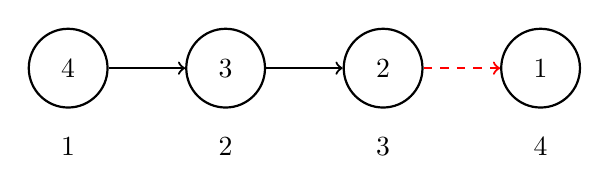
\begin{tikzpicture}[thick]
        \edef\pos{0}
        \foreach \x in {1, 2,..., 4}{
            \pgfmathparse{\pos+2}
            \xdef\pos{\pgfmathresult}
            \node  at (\pos, -1) {$\x$};
        }
        \node[circle,draw, minimum size=1cm] (1) at  (2, 0) {$4$};
        \node[circle,draw, minimum size=1cm] (2) at  (4, 0) {$3$};
        \node[circle,draw, minimum size=1cm] (3) at  (6, 0) {$2$};
        \node[circle,draw, minimum size=1cm] (4) at  (8, 0) {$1$};
        \draw[->] (1) -- (2);
        \draw[->] (2) -- (3);
        \draw[->, color=red, dashed] (3) -- (4);
    \end{tikzpicture}
    \caption[Exemplo de expiração de certificado da lista ordenada]{No exemplo da
    Figura~\ref{fig:ordenacao:exemplo}, \cert[3] expirou no instante $t = 2$.}
    \label{fig:lista:expire}
\end{figure}

\begin{figure}
    \centering
    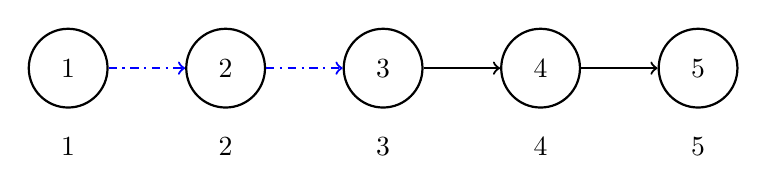
\begin{tikzpicture}[thick]
        \edef\pos{0}
        \foreach \x in {1, 2,..., 5}{
            \pgfmathparse{\pos+2}
            \xdef\pos{\pgfmathresult}
            \node[circle,draw, minimum size=1cm] (\x) at
                (\pos, 0) {$\x$};
            \node  at (\pos, -1) {$\x$};
        }
        % \foreach \x [evaluate=\x as \y using int(\x + 1)] in {1, 2,..., 4}{
        %     \ifthenelse{\x==2}{\draw[->, draw=red] (\x) -- (\y);}{\draw[->, draw=black] (\x) -- (\y);}
        % }
        \draw[->, color=blue, dashdotted] (1) -- (2);
        \draw[->, color=blue, dashdotted] (2) -- (3);
        \draw[->] (3) -- (4);
        \draw[->] (4) -- (5);
        % \draw[->] (1) edge (2) (2) edge (3) (3) edge (4) (4) edge (5)
    \end{tikzpicture}
    \caption[Certificados atualizados]{Após a mudança de velocidade
            do elemento 2, que se encontra em \sorted[2], \cert[1] e
            \cert[2] foram atualizados.}
    \label{fig:lista:after}
\end{figure}

A operação \textsc{query\_max}, no Algoritmo \ref{torn:querymax},
consiste em devolver \torneio$[1]$, enquanto que a operação
\textsc{change}$(j, v)$, no Algoritmo \ref{torn:change}, consiste em
alterar a posição $x_0[j]$ para ${x_0[j] + (\mathit{speed}[j] -
v)\cdot now}$, a posição \textit{speed}$[j]$ para \textit{v} e
recalcular os eventuais certificados de que $j$ participa. Para
tanto, a partir da posição $i$ em que $j$ se encontra no vetor
\torneio, podemos recalcular \textit{cert}$[j]$ e então continuamos
visitando as partidas em que $j$ participou para atualizar os
certificados daqueles que perderam de $j$, acionando a rotina
\textsc{update} para fazer os devidos acertos em $Q$ correspondentes
a estas modificações.

\begin{algorithm}
    \caption{Função \textsc{query\_max}.} \label{torn:querymax}
    \begin{algorithmic}[1]
        \Function{query\_max}{\nnull}
            \State \Return \torneio$[1]$
        \EndFunction
    \end{algorithmic}
\end{algorithm}

\begin{algorithm}
    \caption{Função \textsc{change}.} \label{lista:change}
\begin{algorithmic}[1]
    \Function{change}{$j, v$}
        \State $x_0$[$j$] $\leftarrow  x_0$[$j$]
        $+~($\speed[$j$]$~-~v)~\cdot~$\now;
        \State \speed[$j$] $\leftarrow  v$
        \State $i \leftarrow$ \inds[$j$]
        \State \Call{update}{$i$}
        \State \Call{update}{$i - 1$}
    \EndFunction
\end{algorithmic}
\end{algorithm}

\begin{algorithm}
    \caption{Função \textsc{change}.} \label{lista:change}
\begin{algorithmic}[1]
    \Function{change}{$j, v$}
        \State $x_0$[$j$] $\leftarrow  x_0$[$j$]
        $+~($\speed[$j$]$~-~v)~\cdot~$\now;
        \State \speed[$j$] $\leftarrow  v$
        \State $i \leftarrow$ \inds[$j$]
        \State \Call{update}{$i$}
        \State \Call{update}{$i - 1$}
    \EndFunction
\end{algorithmic}
\end{algorithm}

%!TeX root=./torneio.tex

\subsection{Inserção e remoção em torneio} \label{trni:secao}

Assim como fizemos na seção \ref{abb}, além das operações
\textsc{advance}$(t)$, \textsc{change}$(j, v)$ e
\textsc{query\_max}$()$ poderíamos querer dar suporte a operações
como:

\begin{itemize}
    \item \textsc{insert}$(v, x_t)\rightarrow$ insere um elemento
    com velocidade $v$ e valor $x_t$ no instante \now;
    \item \textsc{delete}$(i) \rightarrow$ remove o elemento $i$ no
    instante \now.
\end{itemize}
Agora, diferentemente da seção \ref{abb}, não utilizaremos uma nova
estrutura para dar suporte à essas operações, pois um torneio já
suporta operações como inserção e remoção de elementos em tempo
logarítmico. Porém, da maneira como se encontra a interface,
poderíamos ter problemas como espaços de memória ociosos após várias
remoções ou um gasto elevado de tempo redimensionando vetores para
que suportem a inserção de novos elementos. Dessa forma,
descreveremos a seguir alterações a serem feitas na interface para
evitar problemas como os citados.

Inicialmente o vetor que guarda o torneio começa com os elementos
ocupando as suas últimas posições e construímos o torneio de acordo
com o valor de cada elemento no instante $t = 0$.

Uma vez de posse do torneio montado, construímos um certificado para
cada elemento no torneio. Agora os certificados não serão mais
mantidos em um vetor; serão mantidos junto dos elementos para
facilitar a inserção e remoção de certificados, já que estas vêm
junto com a inserção e remoção de elementos. O certificado de um
elemento $e$ se refere à relação estabelecida entre o elemento $e$ e
o elemento $k$, que é o elemento que venceu $e$ na última partida
que $e$ disputou, consiste no instante de tempo em que o elemento
$e$ passará a ter um valor maior que o valor do elemento $k$, se
esse instante for maior que o instante atual. Do contrário, o
certificado consiste em $+\infty$.

Note que o elemento que está na primeira posição do torneio não é
vencido por ninguém no instante \now. Portanto, daremos o valor
$+\infty$ para o seu certificado.

Esses $n$ certificados serão colocados em uma fila de prioridade,
com o prazo de validade como chave. O certificado com menor prazo de
validade estará ocupando a primeira posição da fila. Na verdade,
como os certificados estarão diretamente ligados aos elementos,
colocaremos os elementos na fila de prioridade. Além disso, a
interface da fila de prioridade passará a suportar as operações
\textsc{insertPQ}$(Q, e)$ e \textsc{deletePQ}$(Q, e)$.

Para descrever as implementações das operações, vamos estabelecer os
nomes dos objetos, variáveis e rotinas auxiliares utilizados:
\begin{enumerate}
    \item $n$: número de elementos no instante \now;
    \item \elemento: objeto com os seguintes atributos:
    \begin{enumerate}
        \item \id: atributo para identificar o objeto.
        Daqui em diante, usaremos elemento $i$ para se referir
        ao elemento cujo \id~é $i$;

        \item \speed: a velocidade do elemento;

        \item \initv: é o valor que o elemento possuía no
        instante $t = 0$;

        \item \cert: o tempo de validade do certificado do
        elemento;

        \item \pqpos: atributo que aponta para a posição do
        elemento na fila de prioridade;

        \item \lastmatch: atributo que aponta para a posição do
        vetor \torneio~em que o elemento disputou sua última
        partida.
    \end{enumerate}
    \item \torneio: vetor, de $2n - 1$ posições, que guarda
    apontadores para os elementos formando um torneio de acordo com
    seus valores no instante \now;

    \item \Q: fila de prioridade que contém os elementos, o elemento
    com certificado de menor valor estará a frente da fila;

    \item \textsc{insertTourn}$(e) \rightarrow$ insere $e$, que é um
    elemento, no torneio e atualiza os certificados necessários no
    processo;

    \item \textsc{deleteTourn}$(e) \rightarrow$ remove $e$, que é um
    elemento, do torneio e atualiza os certificados necessários no
    processo.
\end{enumerate}
Para a implementação das operações \textsc{change}$(j, v)$ e
\textsc{delete}$(i)$ precisamos de alguma maneira recuperar um
elemento baseado no seu \id. Para tal, podemos utilizar estruturas
como uma árvore de busca binária balanceada ou uma tabela de
dispersão. A seguir~estão três operações que nos ajudarão a
recuperar os elementos:
\begin{enumerate}
    \item \textsc{getObject}$(i)\rightarrow$ retorna o elemento $i$;
    \item \textsc{insertObject}$(e) \rightarrow$ insere $e$, que é
    um elemento, na estrutura;
    \item \textsc{deleteObject}$(e) \rightarrow$ remove $e$, que é
    um elemento, da estrutura.
\end{enumerate}
Para permitir a inserção e remoção de certificados, a interface da
fila de prioridade será reformulada, contando com duas operações
extras:
\begin{enumerate}
    \item \textsc{insertPQ}$(Q, e) \rightarrow$ insere $e$ na fila
    de prioridade $Q$;
    \item \textsc{deletePQ}$(Q, e) \rightarrow$ remove $e$ da fila
    de prioridade $Q$;
    \item \textsc{updatePQ}$(Q,e,t) \rightarrow$ muda o valor do
    certificado de $e$ para $t$ e atualiza a fila de prioridade $Q$;
    \item \textsc{minPQ}$(Q) \rightarrow$ devolve o elemento com o
    certificado de menor valor da fila de prioridade $Q$.
\end{enumerate}
A operação \textsc{updatePQ}$(Q,e,t)$ pode ser implementada em tempo
logarítmico graças ao atributo \pqpos~dos elementos.

Um evento está associado a um certificado $(e, t)$ que expira no
instante $t$. Na implementação da operação \textsc{event},
utilizaremos a rotina \textsc{update}$(e)$, do algoritmo
\ref{torneioi:update}, que calcula a nova validade $t$ do
certificado do elemento $e$, e chama a rotina $\textsc{updatePQ}(Q,
e, t)$.

\begin{algorithm}[H]
    \caption{Função \textsc{update}.} \label{torneioi:update}
    \begin{algorithmic}[1]
        \Function{update}{$e$}
            \If{$e \neq$ NULL}
                \State $e'\leftarrow \torneio[(e.\lastmatch)/2]$
                \State $t \leftarrow $ \Call{expire}{$e, e'$}
                \State \Call{updatePQ}{$Q,e,t$}
            \EndIf
        \EndFunction
        % \LineComment{Em expire$(e, e')$, $e'$ pode ser nulo e
        % nesse caso o retorno é $+\infty$.}
        % \LineComment{\Call{expire}{$e,e'$} calcula a validade do
        % certificado entre os elementos $e$ e $e'$, se $e'$ é NULL
        % retorna $+\infty$}
    \end{algorithmic}
\end{algorithm}

\begin{algorithm}[H]
    \caption{Função \textsc{event}.} \label{torneioi:evento}
    \begin{algorithmic}[1]
        \Function{event}{\nnull}
            \State $e \leftarrow  $ \Call{minPQ}{$Q$}
            \While{$e.\cert$ = \now}
                \State $j \leftarrow e.\lastmatch$
                \State $k \leftarrow 2\cdot \floor{\frac{j}{2}}
                + ((j + 1)\mod2)$ \Comment{adversário}
                \While{$j > 1$ \AND \Call{value}{$j$} $\geq$
                    \Call{value}{$k$}}
                    \State \torneio[$\floor{\frac{j}{2}}$]
                    $\leftarrow~$\torneio[$j$]
                    \State $\torneio[k].\lastmatch$ $\leftarrow k$
                    \State \Call{update}{$\torneio[k]$}
                    \State $j \leftarrow \floor{\frac{j}{2}}$
                    \State $k \leftarrow 2\cdot \floor{\frac{j}{2}}
                    + ((j + 1)\mod2)$ \Comment{adversário}
                \EndWhile
                \State $\torneio[j].\lastmatch \leftarrow j$
                \State \Call{update}{$\torneio[j]$}
                \State $e \leftarrow  $ \Call{minPQ}{$Q$}
            \EndWhile
        % \LineComment{swapHeap$(i, \floor{\frac{i}{2}})$ troca \heap[$i$] por \heap$\left[\floor{\frac{i}{2}}\right]$}
        \EndFunction
%        \LineComment{\Call{compare}{$i, j$} retorna se o valor
%        de $i$ é maior que o valor de $j$.}
    \end{algorithmic}
\end{algorithm}

No trecho das linhas 5 - 11 do código \ref{torneioi:evento}, o
resultado da partida entre o elemento~$j$ e seu adversário que se
encontra na posição $k$ de \torneio~é recalculado, e o certificado
correspondente é atualizado. Caso o resultado da partida tenha sido
alterado, a verificação se propaga para o nível de cima.

A operação \textsc{query\_max}$()$, no algoritmo
\ref{torneioi:query}, consiste em devolver \torneio$[1]$, enquanto
que a operação \textsc{change}$(j, v)$ consiste em recuperar o
elemento~$j$, alterar seu atributo \initv~para
$x_0+(\mathit{speed}-v)\cdot now$, \textit{speed} para \textit{v} e
recalcular os eventuais certificados de que $j$ participa. Para
tanto, a partir da posição $i$ mais alta em que $j$ se encontra no
vetor \torneio, podemos recalcular \textit{cert}$[j]$ e então
continuamos visitando as partidas em que $j$ participou para
atualizar os certificados daqueles que perderam de $j$, acionando a
rotina \textsc{updatePQ} para fazer os devidos acertos em $Q$
correspondentes a estas modificações.

\begin{algorithm}
    \caption{Função \textsc{query\_max}.} \label{torn:querymax}
    \begin{algorithmic}[1]
        \Function{query\_max}{\nnull}
            \State \Return \torneio$[1]$
        \EndFunction
    \end{algorithmic}
\end{algorithm}

\begin{algorithm}
    \caption{Função \textsc{change}.} \label{lista:change}
\begin{algorithmic}[1]
    \Function{change}{$j, v$}
        \State $x_0$[$j$] $\leftarrow  x_0$[$j$]
        $+~($\speed[$j$]$~-~v)~\cdot~$\now;
        \State \speed[$j$] $\leftarrow  v$
        \State $i \leftarrow$ \inds[$j$]
        \State \Call{update}{$i$}
        \State \Call{update}{$i - 1$}
    \EndFunction
\end{algorithmic}
\end{algorithm}

A operação \textsc{insert}$(v, x_t)$ consiste em criar um novo elemento,
inicializando seus atributos com os devidos valores,
inseri-lo no torneio e na estrutura que usamos para recuperá-lo,
calcular o seu certificado e inseri-lo na fila de prioridade.
Uma importante observação é que se \now~$\neq 0$, então $x_t
\neq$~\initv. Para calcular \initv, podemos utilizar a relação
$x_t = now\cdot speed + x_0 \Rightarrow x_0 = x_t - speed\cdot
now$.

\begin{algorithm}
    \caption{Função \textsc{insert}.} \label{torneioi:insert}
    \begin{algorithmic}[1]
        \Function{insert}{$v, x_t$}
            \State $e.speed \leftarrow v$
            \State $e.x_0 \leftarrow x_t - now\cdot v$
            \State \raiz~$\leftarrow$ \Call{insertObject}{$root, e$}
            \State \Call{insertTourn}{$e$}
            \State \Call{newCert}{$e$}
            \State \Call{insertPQ}{$Q, e$}
        \EndFunction
    \end{algorithmic}
\end{algorithm}

A operação \textsc{delete}$(i)$ consiste em recuperar o
elemento~$i$, removê-lo da fila de prioridade, do torneio e da
estrutura que usamos para recuperá-lo depois.

\begin{algorithm}
    \caption[Algoritmo \textsc{delete} da árvore binária de busca]{Função \textsc{delete}.} \label{alg:abb:delete}
    \begin{algorithmic}[1]
        \Function{delete}{$i$}
            \State $e \leftarrow$ \Call{getObject}{$i$}
            \State $e' \leftarrow e.next$
            \State \raiz~$\leftarrow$ \Call{deleteKey}{$\raiz, e$}
            \State \Call{deleteObject}{$e$}
            \State \Call{deletePQ}{$Q, e$}
            \State \Call{update}{$e'$}
        \EndFunction
    \end{algorithmic}
\end{algorithm}

A função auxiliar \textsc{insertTourn}$(e)$, do algoritmo
\ref{torneioi:insert}, consiste de criar uma nova partida, usando o
elemento que está na posição $n$ para completar a partida, depois
subimos para o nível de cima no torneio, corrigindo os vencedores
das partidas e atualizando os certificados correspondentes. O
certificado do elemento inserido não será calculado nessa função,
será calculado posteriormente. Na implementação do algoritmo
\ref{torneioi:inserttourn}, $\textsc{resize}()$ checa se \torneio~é
capaz de suportar a inserção de novos elementos e, se não for,
redimensiona \torneio.

\begin{algorithm}[H]
    \caption{Função \textsc{insertTourn}.} \label{torneioi:inserttourn}
    \begin{algorithmic}[1]
        \Function{insertTourn}{$e$}
            \State \Call{resize}{\nnull}
            \State $n \leftarrow n + 1$
            \State $i \leftarrow 2n - 1$
            \State $\torneio[i] \leftarrow e$
            \State $\torneio[i - 1] \leftarrow \torneio[\floor{i/2}]$
            \State $k \leftarrow i - 1$
            \While{$i > 1$ \AND \Call{value}{$i$} $\geq$
                \Call{value}{$k$}}
                \State $\torneio[\floor{i/2}] \leftarrow \torneio[i]$
                \State $\torneio[k].\lastmatch \leftarrow k$
                \State \Call{update}{$\torneio[k]$}
                \State $i \leftarrow \floor{i/2}$
                \State $k \leftarrow 2\cdot \floor{i/2} +
                ((i + 1)\mod2)$ \Comment{adversário}
            \EndWhile
            \State $\torneio[1].\lastmatch \leftarrow 1$
        \EndFunction
    \end{algorithmic}
\end{algorithm}

\begin{figure}
    \centering
        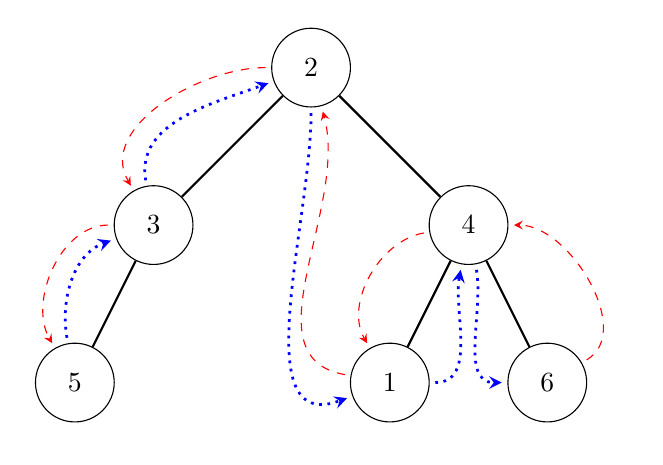
\begin{tikzpicture}[baseline=-2.25cm]
            \node[circle,draw,minimum size=1cm] (1) at (0,0)  {$2$};
            \node[circle,draw,minimum size=1cm] (2) at (-2,-2){$3$};
            \node[circle,draw,minimum size=1cm] (3) at (2,-2) {$4$};
            \node[circle,draw,minimum size=1cm] (4) at (-3,-4){$5$};
            \node[circle,draw,minimum size=1cm] (5) at (1,-4) {$1$};
            \node[circle,draw,minimum size=1cm] (6) at (3,-4) {$6$};
            % \node[label={7},circle,draw,minimum size=1cm] (7) at (3,-4) {$8$};
            % \node[label={8},circle,draw,minimum size=1cm] (8) at (-4,-6) {$4$};
            % \node[label={9},circle,draw,minimum size=1cm] (9) at (-2,-6) {$1$};
            \tikzstyle{filho}=[thick]
            \tikzstyle{pred}=[->, shorten >= 2pt, shorten <= 2pt,
                    dashed, >=stealth, red]
            \tikzstyle{sucessor}=[->, shorten >= 2pt, shorten <= 2pt,
                    dotted, >=stealth, blue, line width=0.35mm]
            % \tikzstyle{p4}=[->, shorten >= 2pt, shorten <= 2pt, dotted, >=stealth]
            \draw[filho] (1) -- (2);
            \draw[filho] (1) -- (3);
            \draw[filho] (2) -- (4);
            \draw[filho] (3) -- (5);
            \draw[filho] (3) -- (6);
            \draw[pred] (6) edge[out=30,in=0] (3);
            \draw[sucessor] (3) edge[out=280,in=180] (6);
            \draw[pred] (3) edge[out=190,in=120] (5);
            \draw[sucessor] (5) edge[out=0,in=260] (3);
            \draw[pred] (5) edge[out=170,in=285] (1);
            \draw[sucessor] (1) edge[out=270,in=200] (5);
            \draw[pred] (1) edge[out=180,in=120] (2);
            \draw[sucessor] (2) edge[out=100,in=200] (1);
            \draw[pred] (2) edge[out=180,in=120] (4);
            \draw[sucessor] (4) edge[out=100,in=200] (2);
        \end{tikzpicture}
        \qquad
        \qquad
        \qquad
        \begin{tabular}{|c|c|}
            \hline
            $i$ & $x_0$ \\
            \hline
            $1$ & $6$ \\

            $2$ & $3$ \\

            $3$ & $2$ \\

            $4$ & $7$ \\

            $5$ & $-2$ \\

            $6$ & $14$ \\
            \hline
        \end{tabular}
        \caption[Exemplo de estrutura da ABB]{Exemplo de árvore em
            que a ordem dos elementos, do menor para o maior no
            instante $\now = 0$, é $5 - 3 - 2 - 1 - 4 - 6$. Os
            apontadores para o elemento anterior são representados
            pelas setas vermelhas tracejadas e os apontadores para o
            elemento posterior são representados pelas setas azuis
            pontilhadas.}\label{fig:abb:exemplo}
\end{figure}

\begin{algorithm}
    \caption{Função \textsc{insert}.} \label{torneioi:insert}
    \begin{algorithmic}[1]
        \Function{insert}{$v, x_t$}
            \State $e.speed \leftarrow v$
            \State $e.x_0 \leftarrow x_t - now\cdot v$
            \State \raiz~$\leftarrow$ \Call{insertObject}{$root, e$}
            \State \Call{insertTourn}{$e$}
            \State \Call{newCert}{$e$}
            \State \Call{insertPQ}{$Q, e$}
        \EndFunction
    \end{algorithmic}
\end{algorithm}

A função auxiliar \textsc{deleteTourn}$(e)$, do algoritmo
\ref{torneioi:delete}, consiste de usar o perdedor
da partida travada entre os elementos que estão nas duas últimas
posições de \torneio~para substituir o elemento $e$.
Além disso, desfazemos essa partida para que os
$n$ elementos continuem a ocupar as $2n - 1$ primeiras posições
do torneio após a remoção de $e$. O perdedor
substituíra o elemento $e$ na posição da
primeira partida de que $e$ participou. Todas as partidas desde
essa posição, se propagando para o nível de cima no caminho até a
primeira posição, serão recalculadas com os devidos certificados
atualizados. Essa propagação até a primeira posição é importante
para que não hajam resquícios do elemento deletado no torneio,
veja o exemplo da figura \ref{fig:torneioi:delete}. Na implementação,
no algoritmo \ref{torneioi:deletetourn}, \textsc{substitute}$(e)$ faz a
substituição citada retornando a posição da primeira partida
de que $e$ participou.

\begin{algorithm}
    \caption{Função \textsc{deleteTourn}.} \label{torneioi:deletetourn}
    \begin{algorithmic}[1]
        \Function{deleteTourn}{$e$}
            \State $i \leftarrow $ \Call{substitute}{$e$}
            \State $k \leftarrow 2\cdot \floor{i/2} + ((i + 1)\mod2)$
            \While{$i > 1$}
                \If{\Call{compare}{$k, i$}}
                    \State $i \leftrightarrow k$
                \EndIf
                \State $\torneio[\floor{i/2}] \leftarrow \torneio[i]$
                \State $\torneio[k].\lastmatch \leftarrow k$
                \State \Call{update}{$\torneio[k]$}
                \State $i \leftarrow \floor{i/2}$
                \State $k \leftarrow 2\cdot \floor{i/2} + ((i + 1)\mod2)$
                \Comment{adversário}
            \EndWhile
            \State $\torneio[1].\lastmatch \leftarrow 1$
                \State \Call{update}{$\torneio[1]$}
        \EndFunction
    \end{algorithmic}
\end{algorithm}

\begin{algorithm}
    \caption[Algoritmo \textsc{delete} da árvore binária de busca]{Função \textsc{delete}.} \label{alg:abb:delete}
    \begin{algorithmic}[1]
        \Function{delete}{$i$}
            \State $e \leftarrow$ \Call{getObject}{$i$}
            \State $e' \leftarrow e.next$
            \State \raiz~$\leftarrow$ \Call{deleteKey}{$\raiz, e$}
            \State \Call{deleteObject}{$e$}
            \State \Call{deletePQ}{$Q, e$}
            \State \Call{update}{$e'$}
        \EndFunction
    \end{algorithmic}
\end{algorithm}
